%!TEX root = ../document.tex

\section{Method of Rocha et al.}
\label{sec:section2}

The method proposed by Rocha et al. is divided into three stages: preprocessing, feature extraction and classification/detection. The key points of the methodology are (i) a measure of ST deviation based on time-frequency analysis of the ECG signal and (ii) expansion of the QRS complex and T wave morphologies onto Hermite basis functions. Figure \ref{fig:rocha_01} shows a high-level block diagram of the strategy adopted.

\begin{figure}[h]
    \centering
    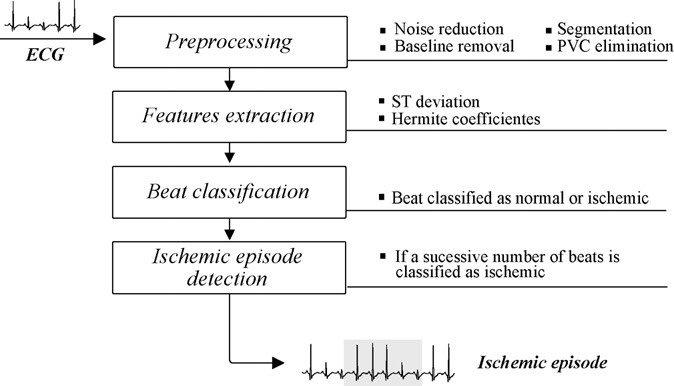
\includegraphics[width=0.6\textwidth]{figures/rocha_01.png}
    \caption[Rocha strategy block diagram]
    {High-level block diagram of the strategy used in Rocha}
    \label{fig:rocha_01}
\end{figure}

\subsection{Preprocessing}
    In this stage, a discrete input signal containing the normalized amplitudes\footnote{here, normalized means $(SignalAmplitude - VerticalOffset) / VoltageGain$} of an ECG lead is processed for (i) noise suppression, (ii) segmentation into characteristic waves, (iii) elimination of premature ventricular contractions and (iv) baseline removal. Implementation of these procedures is detailed below.
    
    \subsubsection{Noise suppression}
    \subsubsection{Segmentation}
    \subsubsection{PVC elimination}
    \subsubsection{Baseline removal}
    
\subsection{Feature extraction}
    In this stage, two groups of features are drawn from the ECG signal, namely the ST segment shift estimation and the Hermite expansion of QRS complex and T waves. In the first group, changes in ST segment shift measured from the baseline are used to discriminate ischemic from non-ischemic beats. In the second group, changes in QRS complex and in T wave morphologies are also indicators of ischemic or normal beats.
    
    \subsubsection{ST segment deviation based on R peak location}
    \subsubsection{ST segment deviation based on time-frequency analysis}
    \subsubsection{QRS complex and T wave characterization}
    \subsubsection{Expansion in Hermite functions}
    
\subsection{Classification and detection}
    In this stage\ldots
    
    \subsubsection{Ischemic ST elevation}
    \subsubsection{Ischemic ST depression}
    \subsubsection{Ischemic episode detection}
    
\subsection{Results}
    To assess the performance of the algorithm, we use the concepts of sensibility and positive predictivity, which are calculated based on the number of true positives (TP), true negatives (TN), false positives (FP) and false negatives (FN) given by a diagnostic test. Here, sensibility is the ratio of cardiac beats correctly identified as ischemic to the number of truly ischemic beats ($TP/(TP+FN)$), whereas positive predictivity is the ratio of cardiac beats correctly identified as ischemic to the number of beats diagnosed as ischemic ($TP/(FP+TP)$).
    
    With this definition, one can say that sensibility is a measure of how rarely the test misses actual ischemic beats, whereas positive predictivity is a measure of how optimistic -- in the ironic sense of diagnosing ischemic beats -- the test is with respect to the set of samples. We shall use the same concepts in the forthcoming sections.
